\chapter{Psalm 3}

\begin{figure}
  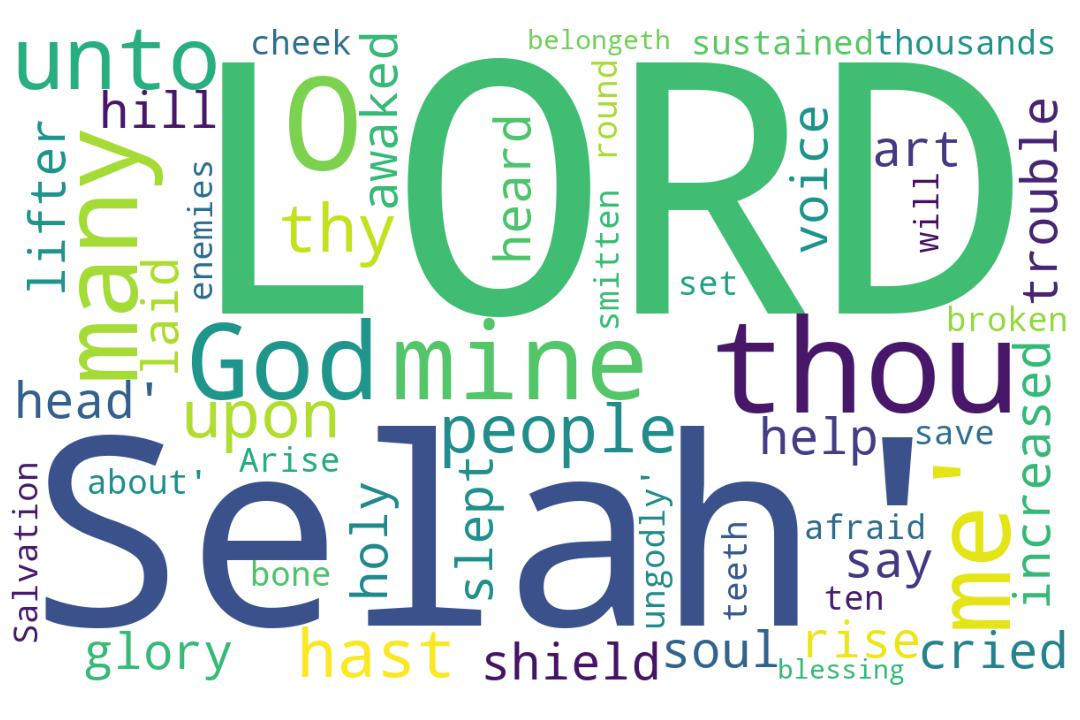
\includegraphics[width=\linewidth]{19OT-Psalms/Psalm3-WordCloud.jpg}
  \caption{Psalm 3 Word Cloud}
  \label{fig:Psalm 3 word Cloud}
\end{figure}

\marginpar{\scriptsize \centering \fcolorbox{bone}{lime}{\textbf{THE LORD, MY HELP}}\\ (Psalm 3:1-8) \begin{compactenum}[I.][8]
	\item A \textbf{Distressed Soul} \index [scripture]{Psalms!Psa 003:02} (Psa 3:2)
	\item A \textbf{Durable Shield} \index [scripture]{Psalms!Psa 003:03} (Psa 3:3)
	\item A \textbf{Defender \& Sustainer} \index[scripture]{Psalms!Psa 003:05} (Psa 3:5)
    \item \textbf{Delightful Sleep} of Peace \index[scripture]{Psalms!Psa 003:05} (Psa 3:5)
    \item One \textbf{Dependable \& Sure} \index[scripture]{Psalms!Psa 003:06} (Psa 3:6)
    \item \textbf{Determined \& Smiting} \index[scripture]{Psalms!Psa 003:07} (Psa 3:7)
   \item  \textbf{Deliverer of Salvation} \index[scripture]{Psalms!Psa 003:08} (Psa 3:8)
\end{compactenum} }

\marginpar{\scriptsize \centering \fcolorbox{bone}{yellow}{\textbf{WHAT GOD DID FOR DAVID}}\\ (Psalm 3:1-8) God:
\begin{compactenum}[I.][8] 
    \item \textbf{God Saw him Surrounded by Enemies} \index[scripture]{Psalms!Psa 003:01} (Psa 3:1)
    \item \textbf{God Secured Him Against Overwhelming Odds} \index[scripture]{Psalms!Psa 003:01} (Psa 3:1)
    \item \textbf{God Sent him Help} \index[scripture]{Psalms!Psa 003:02} (Psa 3:2)
    \item \textbf{God Shielded him from Hurt} \index[scripture]{Psalms!Psa 003:03} (Psa 3:3)
    \item \textbf{God Sustained Him} \index[scripture]{Psalms!Psa 003:05} (Psa 3:5)
    \item \textbf{God Smote the Heathen} \index[scripture]{Psalms!Psa 003:07} (Psa 3:7)
    \item \textbf{God Separated the Teeth of the ungodly} \index[scripture]{Psalms!Psa 003:07} (Psa 3:7)
\end{compactenum} }

\marginpar{\scriptsize \centering \fcolorbox{bone}{black}{\textbf{\textcolor[cmyk]{0,0,0,0}{A TIME OF ANGUISH}}}\\ (Psalm 3) 
\begin{compactenum}[I.]
    \item \textbf{Personal Heartache} - - and heartbreak, but by God's grace and mercy, it was also a time of:
    \item \textbf{Persistent Help} (verses 3, 4, 5, 7)
    \item \textbf{Protected Head} - - God protected both David's physical head and David's throne, the headship as king (verse 3)
    \item A \textbf{Penitential Heart} - - no doubt that David fully realized that Absalom's rebellion, along with many other family problems, results from his sin with Bathsheba. David was never the same after this succession of sin.  He lived with his sorrow.
    \item \textbf{Purifying and Healing} - - there is nothing like God letting us reap the seed we have sown to let us experience his mercy. It is both a purifying and healing process to go through this.  God delivers and cleanses, yet again. 
    \item \textbf{Preserved Honor} - - David gets restored back to the throne, and Absalom is killed by Joab
    \item An \textbf{Ever-Present Hope}
\end{compactenum} }

\marginpar{\scriptsize \centering \fcolorbox{bone}{blue}{\textbf{\textcolor[cmyk]{0,0,0,0}{READYING THE PLACE}}}\\
\fcolorbox{bone}{blue}{\textbf{\textcolor[cmyk]{0,0,0,0}{OF REFUGE}}} \\(Psalm 3) \\
Psalm 3 has the second mention of this word ``Selah''. The first is in 2 Kings 14:7, where it is captured and given the name ``Joktheel.''
\begin{compactenum}[I.]
    \item The \textbf{Capture} - \index[scripture]{2Kings!2Ki 14:07} (2 Kings 14:7)
    \item The \textbf{Coalition} - \index[scripture]{Psalms!Psa 003:01} (Psa 3:1)
    \item The \textbf{Condition} - \index[scripture]{Psalms!Psa 003:02} (Psa 3:2)
    \item The \textbf{Cry} - \index[scripture]{Psalms!Psa 003:04} (Psa 3:4)
    \item The \textbf{Care} - \index[scripture]{Psalms!Psa 003:04} (Psa 3:5)
     \item The \textbf{Conquest} - \index[scripture]{Psalms!Psa 003:07} (Psa 3:7)
   \item The \textbf{Consummation} - \index[scripture]{Psalms!Psa 003:08} (Psa 3:8)
\end{compactenum} }

\footnote{\textcolor[cmyk]{0.99998,1,0,0}{\hyperlink{TOC}{Return to end of Table of Contents.}}}\footnote{\href{https://www.audioverse.org/english/audiobibles/books/ENGKJV/O/Ps/1}{\textcolor[cmyk]{0.99998,1,0,0}{Psalms Audio}}}\textcolor[cmyk]{0.99998,1,0,0}{A Psalm of David, when he fled from Absalom his son.}\\
\\
\textcolor[cmyk]{0.99998,1,0,0}{LORD\textcolor{jungle}{$_{337}$}, how are they increased that trouble me! many \emph{are} they that rise up against me.}
[2] \textcolor[cmyk]{0.99998,1,0,0}{Many\textcolor{jungle}{$_{353}$} \emph{there} \emph{be} which say of my \fcolorbox{bone}{lime}{soul}, \emph{There} \emph{is} no help for him in God. Selah.}
[3] \textcolor[cmyk]{0.99998,1,0,0}{But\textcolor{jungle}{$_{370}$} thou, O LORD, \emph{art} a \fcolorbox{bone}{lime}{shield} for me; my glory, and the lifter up of mine head.}
[4] \textcolor[cmyk]{0.99998,1,0,0}{I\textcolor{jungle}{$_{388}$} cried unto the LORD with my voice, and he heard me out of his holy hill. Selah.}
[5] \textcolor[cmyk]{0.99998,1,0,0}{I\textcolor{jungle}{$_{406}$} laid me down and \fcolorbox{bone}{lime}{slept}; I awaked; for the LORD \fcolorbox{bone}{lime}{sustained} me.}
[6] \textcolor[cmyk]{0.99998,1,0,0}{I\textcolor{jungle}{$_{419}$} will \fcolorbox{bone}{lime}{not} be afraid of ten thousands of people, that have set \emph{themselves} against me round about.}
[7] \textcolor[cmyk]{0.99998,1,0,0}{Arise\textcolor{jungle}{$_{437}$}, O LORD; save me, O my God: for thou hast \fcolorbox{bone}{lime}{smitten} all mine enemies \emph{upon} the cheek bone; thou hast broken the teeth of the ungodly.}
[8] \textcolor[cmyk]{0.99998,1,0,0}{\fcolorbox{bone}{lime}{Salvation}\textcolor{jungle}{$_{464}$} \emph{belongeth} unto the LORD: thy blessing \emph{is} upon thy people. Selah\textcolor{jungle}{$_{475}$}.}


